\paragraph{Sơ đồ tuần tự luồng Cập nhật thông tin Cài đặt}

Luồng nghiệp vụ này mô tả
quy trình lưu các thay đổi thiết lập của người dùng
thông qua Setting Service (Neon API).

\begin{figure}[H]
\centering
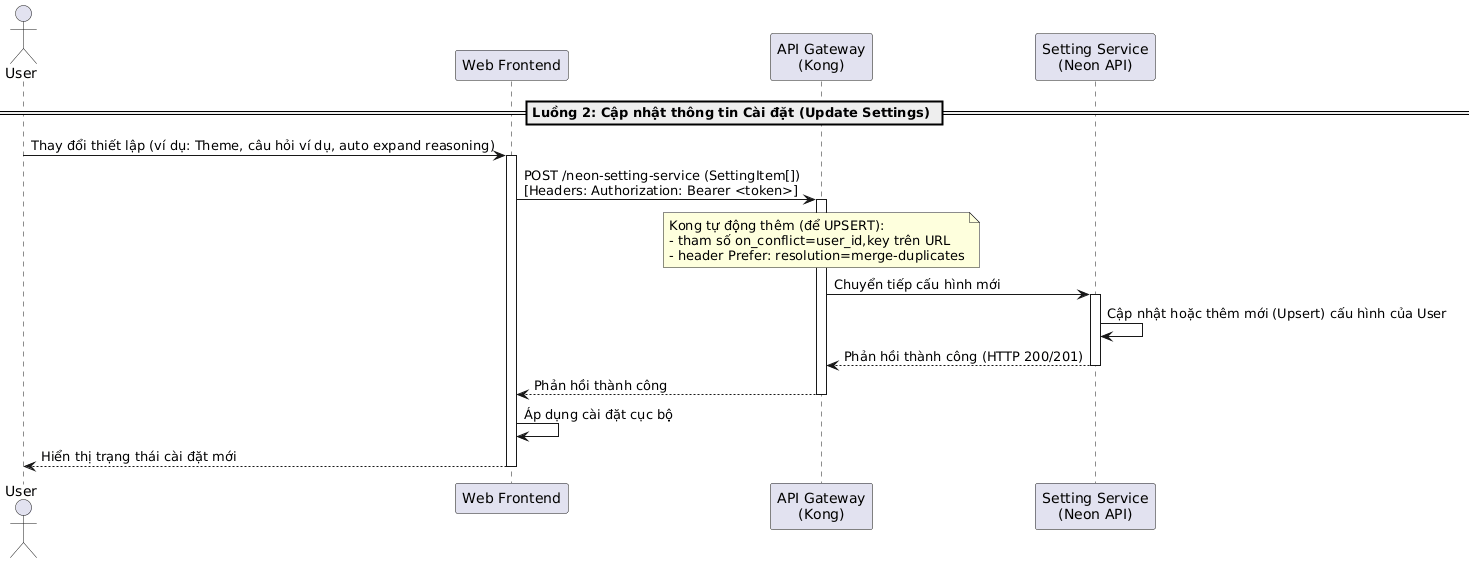
\includegraphics[scale = 0.2]{contents/Sequence/UML-Sequence-UserUpdateSettings.png}
\caption{Sơ đồ tuần tự luồng Cập nhật thông tin Cài đặt}
\end{figure}

\subparagraph{Các thành phần tham gia}

\begin{table}[H]
\centering
\renewcommand{\arraystretch}{1.3}

\begin{tabular}{|l|l|p{5cm}|}
\hline
\textbf{Thành phần} & \textbf{Phân loại} & \textbf{Vai trò trong hệ thống} \\ \hline
User & Actor & Người dùng thực hiện thay đổi cấu hình thiết lập. \\ \hline
Web Frontend & Component & Giao diện web Next.js. \\ \hline %%%% Component & Giao diện Next.js ghi nhận thay đổi, gửi yêu cầu API lưu trữ và áp dụng cài đặt cục bộ. \\ \hline
API Gateway (Kong) & Component & Cổng API chuyển tiếp các yêu cầu API. \\ \hline %%%% Component & Định tuyến yêu cầu cập nhật cài đặt. \\ \hline
Setting Service (Neon API) & Microservice & Dịch vụ tiếp nhận các thiết lập mới, thực hiện cập nhật hoặc thêm mới (Upsert) cấu hình của người dùng. \\ \hline
\end{tabular}
\caption{Các thành phần tham gia luồng Cập nhật thông tin Cài đặt}
\end{table}

\subparagraph{Mô tả tổng quan}

\begin{itemize}
\item \textbf{Thay đổi cài đặt:} Người dùng điều chỉnh các tùy chọn cấu hình trên giao diện cài đặt. Giao diện cập nhật các cài đặt này ở trình duyệt và gửi yêu cầu cập nhật cài đặt qua cổng kết nối đến dịch vụ cấu hình cài đặt.
\item \textbf{Cập nhật cơ sở dữ liệu:} Dịch vụ cấu hình cài đặt thực hiện thêm mới hoặc cập nhật thông tin cài đặt của người dùng vào cơ sở dữ liệu cài đặt.
\item \textbf{Đồng bộ giao diện:} Giao diện cập nhật và hiển thị trạng thái cài đặt mới theo thông tin đã được ghi nhận.
\end{itemize}
